%*******10********20********30********40********50********60********70********80

% For all chapters, use the newdefined chap{} instead of chapter{}
% This will make the text at the top-left of the page be the same as the chapter

\chap{Results}\label{chap:results}
In the following chapter, the numerical results of this study will be displayed and explained. This work was accomplished through the priceless collaboration with Dott. Monasta L. The full discussion will be tackled in Chapter \ref{chap:discussion} on page \pageref{chap:discussion}.

\section{Descriptive analyses}\label{sec:descriptiveanalyses}
As stated in Section \ref{sec:thepopulationinexam}, 285 internationally adopted children were evaluated from January \nth{1}, 2002 to December \nth{31}, 2017; 102 were female (36.17\%) and 180 male (63.83\%). The 3 missing children are due to sex never being registered in the dataset. Males were numerically dominant in all considered regions (55-79\%).\\
The mean ($m$) age at the time of evaluation was 5.2 years (67.8 months), with a standard deviation ($\sigma$) of 2.98 years. The age range spanned from 6 to 156 months. Age overlapped in females and males: for the first group, $m$ was 5.53 and $\sigma$ 3.01; in the latter, $m$ was 5.06 and $\sigma$ 2.97.\\
Moreover, children were evaluated approximately 2 months after their arrival in Italy ($m = 2.23$ and $\sigma = 2.07$).

The evaluated children came from all over the globe, but mostly from Russia ($n = 71$; 25.09\%), India ($n = 43$; 15.19\%), Brazil ($n = 36$; 12.72\%),and Ethiopia ($n = 33$; 11.66 \%). If we were to consider the 4 zones (as defined in Section \ref{sec:thepopulationinexam}), cumulatively, children mostly came from Eastern Europe ($n = 90$; 31.80\%), followed by Latin America ($n = 75$; 26.50\%) and Asia ($n = 72$; 25.44\%); fewer came from Africa ($n = 46$; 16.25\%). Table \ref{fig:populationperyear} shows the growth of our group's size over the years and where these children came from.

117 children out of 271 (43.17\%) had a pathologically underweight, 96 out of 270 (35.55\%) were short for their age.

Haemoglobin was found pathologically low in 22 patients out of 280 (7.86\%). Among these, 9 were moderate, constituting 40.91\% of anemias. Moreover, 9 also presented a pathological MCV and 15 a low ferritin. These findings will be discussed in Section \ref{sec:healthstatusofIAC}.\\
Ferritin was found pathological in 87 out of 251 children (34.66\%): most of these cases were mild deficiencies, but 18 (7.17\%) were very severe. This data can be found in Table \ref{tab:ferritinpatfreq}.

%Begin Table on Ferritin pat freq by region
\begin{table}[H]
   \centering
   \begin{tabular}{l c c c c | r}
   	  & & \multicolumn{3}{c}{Ferritin deficiency} & \\
   	 \cline{3-5}
       & Absent & Mild & Moderate & Severe & Total\\
      \hline
      Frequencies & 164 & 41 & 28 & 18 & 251\\
      Percentages & 65.34\% & 16.33\% & 11.16\% & 7.17\% & 100.00\%\\
   \end{tabular}
   \caption{Absolute frequencies and percentages of ferritin deficiencies in our population.}
    \label{tab:ferritinpatfreq}
\end{table}

As for the immunization status, only 87 (34.25\%) showed a completely valid immunization to vaccine-preventable disease. Almost 65\% of all children was found to have insufficient antibody levels for at least one of the considered diseases. 3 children were \textit{completely} exposed. The following Table \ref{tab:immunizationperregion} shows the immunization status, considered as \textit{complete}, \textit{incomplete} or \textit{absent} for every considered geographical region. Africa resulted being the region with lowest immunization rate (just over $\sim 10\%$).

%Begin Table on Immunization Status by region
\begin{table}[H]
   \centering
   \begin{tabular}{l c c c c | r}
   	  & \multicolumn{3}{c}{Immunization status} & \\
   	 \cline{2-4}
      Region\footnotemark[1] & Absent & Incomplete & Complete & & Totals\\
      \hline
      Africa & 2 (5.56\%) & 30 (83.33\%) & 4 (11.11\%) & & 36\\
      Latin America & 1 (1.47\%) & 44 (64.71\%) & 23 (33.82\%) & & 68\\
      Asia & 1 (1.47\%) & 41 (63.08\%) & 23 (35.38\%) & & 65\\
      Eastern Europe & 0 (0.00\%) & 48 (56.47\%) & 37 (43.53\%) & & 85\\
   \end{tabular}
   \caption{Absolute values and percentages of immunization status of our population, divided by region.}
    \label{tab:immunizationperregion}
\end{table}

\footnotetext[1]{Regions were ordered by the ascending percentage of complete immunization status.}

Out of 285 examined children, on 180 vitamin D serum levels were tested: 60 (33.33\%) were defined deficient, 12 (6.67\%) insufficient, and no children were found to be severely insufficient. Only 108 (60\%) had sufficient (and therefore acceptable) vitamin D intake. Most the children who suffered insufficiency were Asian ($8/12\simeq66.66\%$).\\
The \textit{Kruskal-Wallis equality-of-populations rank test} was performed in order to verify if there were any statistically significant differences in vitamin D mean serum levels between our four zones. Its results were on the limits of statistical significance ($p$-$value=0.0524$). Table \ref{tab:vitamindperregion} shows number of considered cases ($n$), mean serum levels of vitamin D ($m$) and standard deviation ($\sigma$) in each considered region.

%Begin Table on Vitamind D levels per region
\begin{table}[H]
   \centering
   \begin{tabular}{l r r r}
      Region\footnotemark[2] & $n$ & $m$ & $\sigma$\\
      \hline
      Asia & 43 & 19.64 & 9.05\\
      Eastern Europe & 68 & 23.74 & 10.13\\
      Latin America & 39 & 24.20 & 5.87\\
      Africa & 30 & 24.33 & 9.58\\
   \end{tabular}
   \caption{Mean vitamin D serum levels and relative standard deviation in each region in our population.}
    \label{tab:vitamindperregion}
\end{table}

\footnotetext[2]{Regions were ordered by the ascending mean levels of serum vitamin D.}

During our analysis, six countries presented extremely low mean vitamin D serum levels; they are listed in Table \ref{tab:vitamindpercountry}, alongside the number of considered cases per country and the standard deviation.

%Begin Table on Vitamind D levels per country
\begin{table}[H]
   \centering
   \begin{tabular}{l r r r}
      Country\footnotemark[3] & $n$ & $m$ & $\sigma$\\
      \hline
      Ukraine & 1 & 14.00 & -\\
      China & 9 & 15.63 & 7.00\\
      Bulgaria & 2 & 16.00 & 2.97\\
      Romania & 2 & 16.90 & 0.57\\
      Hungary & 3 & 17.63 & 5.29\\
      Benin & 1 & 17.9 & -\\
      Vietnam & 5 & 21.1 & 12.79\\
   \end{tabular}
   \caption{Mean vitamin D serum levels and relative standard deviation of the lowest mean vitamin D values in our population.}
    \label{tab:vitamindpercountry}
\end{table}

\footnotetext[3]{Countries were ordered by the ascending mean levels of serum vitamin D.}

Parasitic gastrointestinal infections were very frequent in our population: 101, out of the total 245 performed tests (41.22\%), resulted positive for at least out of considered intestinal parasites (listed in Section \ref{sub:parasites}). Group 1 parasites were more common in children coming from Latin American and less in Asia; group 2 parasites infected more African children and less Eastern Europeans. None of these results were statistically significant, though: group 1 parasitosis resulted in a 0.105 at the \textit{Fisher's exact test}, group 2 in 0.122. All our data relative to parasitic infections can be found in Table \ref{tab:parasitesperregion}.

%Begin Table on Parasites per region
\begin{table}[H]
   \centering
   \begin{tabular}{l r r c r r}
       & \multicolumn{2}{c}{Group 1} & & \multicolumn{2}{c}{Group 2}\\
       \cline{2-3} \cline{5-6}
      Region\footnotemark[4] & Positive & Negative & & Positive & Negative\\
      \hline
      Asia & 11 (17.74\%) & 51 (82.26\%) & & 13 (20.97\%) & 49 (79.03\%)\\
      Africa & 8 (19.51\%) & 33 (80.49\%) & & 12 (29.27\%) & 29 (70.73\%)\\
      Eastern Europe & 16 (21.62\%) & 58 (78.38\%) & & 9 (12.16\%) & 65 (87.84\%)\\
      Latin America & 25 (34.72\%) & 47 (65.28\%) & & 17 (23.61\%) & 55(76.39\%)\\
      \hline
      Total & 60 (24.10\%) & 189 (75.90\%) & & 51 (20.48\%) & 198 (79.52\%)\\
   \end{tabular}
   \caption{Parasite faecal test result, both absolute and as percentage, divided per region.}
    \label{tab:parasitesperregion}
\end{table}

\footnotetext[4]{Regions were listed in alphabetical order.}

Out of 273 performed Mantoux tests, 46 (16.84\%) resulted positive: a considerable amount. Table \ref{tab:mantouxbyregion} displays all the data on this matter, again, divided by region. Eastern Europe and Africa (as one would expect) resulted to be the region with the highest percentage of positive cases. A \textit{Fisher's exact test} demonstrated a positive statistical correlation between Mantoux test positivity and area of origin ($p$\textless$value=0.002$).

%Begin Table on Mantoux positivity per region
\begin{table}[H]
   \centering
   \begin{tabular}{l r r | r}
   	  & \multicolumn{2}{c}{Mantoux test result} & \\
   	  \cline{2-3}
      Region\footnotemark[5] & Positive & Negative & Total\\
      \hline
      Eastern Europe & 22 (25.29\%) & 65 (74.71\%) & 87 (31.87\%)\\
      Africa & 10 (21.74\%) & 36 (78.26\%) & 46 (16.85\%)\\
      Asia & 11 (15.94\%) & 58 (84.06\%) & 69 (25.27\%)\\
      Latin America & 3 (4.23\%) & 68 (95.77\%) & 71 (26.01\%)\\
      \hline
      Total & 46 (16.85\%) & 227 (83.15\%) & 273 (100.00\%)\\
   \end{tabular}
   \caption{Mantoux test results and relative percentages in each region.}
    \label{tab:mantouxbyregion}
\end{table}

\footnotetext[5]{Regions were ordered by the descending percentage of positive tests.}

The \textit{two-sample Mann-Whitney-Wilcoxon rank-sum test} was performed on each region between Mantoux test results and mean age in the positive and negative groups. It returned a statistically significant ($p$\textgreater$|z|=0.028$) result only for Asia: positive Asiatic children had a mean age of 85 month ($\sigma=31.61$), negative 62 months ($\sigma=37.56$). We believe that with a bigger sample size, this would be found true for Latin America as well.\\
Figure \ref{fig:boxplot_Mantoux} below portrays our population's age distribution (in months) stratified by our four zones and Mantoux test results, perfectly representing this conclusion.

% Mantoux Boxplot
\vspace*{0.8cm}
\begin{figure}[H]
\centering
	\begin{tikzpicture}
		\begin{axis}[
		boxplot/draw direction=y,
		ylabel={Age in months},
		height=8cm,
		xtick pos=left,
		ytick pos=left,
		legend style={area legend, legend columns=-1, anchor=north, at={(0.5,1.15)},column sep=8pt},
		boxplot={
		    %
		    % Idea: 
		    %  place the 
		    %  group 1 at 0.3333 and 0.6666
		    %  group 2 at 1.3333 and 1.6666
		    %  group 3 at 2.3333 and 2.6666
		    %  ...
		    % in a formular:
		    draw position={1/3 + floor(\plotnumofactualtype/2) + 1/3*mod(\plotnumofactualtype,2)},
		    %
		    % that means the box extend must be at most 0.33333 :
		    box extend=0.3,
		},
		% ... it also means that 1 unit in x controls the width:
		x=2.7cm,
		% ... and it means that we should describe intervals:
		xtick={0,1,2,...,10},
		x tick label as interval,
		xticklabels={%
		    {Africa},
		    {Asia},
		    {Eastern Europe},
		    {Latin America},
		},
		    x tick label style={
		        text width=2.8cm,
		        align=center
		    },
		cycle list={{red!70!white},{cyan}},
		every axis plot/.append style={fill,fill opacity=0.3,mark=*}
		]
		
		%Africa
		%Mantoux negativi
		\addplot
		table[row sep=\\,y index=0] {
		data\\
		58\\ 47\\ 18\\ 77\\ 81\\ 42\\ 22\\ 62\\ 19\\ 81\\ 14\\ 55\\ 26\\ 22\\ 56\\ 52\\ 26\\ 26\\ 40\\ 27\\ 55\\ 10\\ 102\\ 41\\ 26\\ 26\\ 11\\ 36\\ 59\\ 120\\ 67\\ 30\\ 75\\ 10\\ 78\\ 90\\
		};
		%Mantoux positivi
		\addplot
		table[row sep=\\,y index=0] {
		data\\
		30\\ 26\\ 20\\ 12\\ 23\\ 87\\ 84\\ 100\\ 81\\ 108\\
		};
		
		%Asia
		%Mantoux negativi
		\addplot
		table[row sep=\\,y index=0] {
		data\\
		57\\ 31\\ 34\\ 141\\ 23\\ 30\\ 49\\ 28\\ 74\\ 78\\ 136\\ 37\\ 17\\ 32\\ 33\\ 16\\ 85\\ 31\\ 87\\ 60\\ 98\\ 60\\ 156\\ 132\\ 132\\ 114\\ 53\\ 96\\ 72\\ 78\\ 78\\ 76\\ 42\\ 21\\ 84\\ 98\\ 69\\ 48\\ 24\\ 84\\ 6\\ 21\\ 62\\ 54\\ 6\\ 119\\ 54\\ 66\\ 108\\ 27\\ 96\\ 32\\ 60\\ 78\\ 7\\ 7\\ 51\\ 75\\
		};
		%Mantoux positivi
		\addplot
		table[row sep=\\,y index=0] {
		data\\
		10\\ 112\\ 86\\ 101\\ 124\\ 80\\ 90\\ 106\\ 80\\ 50\\ 96\\
		};
		
		%Eastern Europe
		%Mantoux negativi
		\addplot
		table[row sep=\\,y index=0] {
		data\\
		58\\ 81\\ 115\\ 36\\ 40\\ 79\\ 85\\ 103\\ 106\\ 50\\ 32\\ 51\\ 74\\ 71\\ 59\\ 81\\ 108\\ 41\\ 38\\ 80\\ 36\\ 54\\ 58\\ 106\\ 102\\ 21\\ 87\\ 64\\ 93\\ 29\\ 27\\ 29\\ 18\\ 26\\ 57\\ 118\\ 94\\ 34\\ 136\\ 84\\ 28\\ 48\\ 108\\ 53\\ 81\\ 13\\ 15\\ 56\\ 36\\ 72\\ 39\\ 112\\ 31\\ 78\\ 78\\ 32\\ 114\\ 92\\ 52\\ 134\\ 16\\ 82\\ 8\\ 28\\ 60\\
		};
		%Mantoux positivi
		\addplot
		table[row sep=\\,y index=0] {
		data\\
		87\\ 23\\ 99\\ 43\\ 91\\ 42\\ 113\\ 74\\ 97\\ 25\\ 44\\ 77\\ 57\\ 66\\ 54\\ 57\\ 75\\ 38\\ 80\\ 126\\ 90\\ 72\\
		};
		
		%Latin America
		%Mantoux negativi
		\addplot
		table[row sep=\\,y index=0] {
		data\\
		76\\ 141\\ 125\\ 90\\ 61\\ 104\\ 91\\ 128\\ 47\\ 101\\ 67\\ 119\\ 151\\ 87\\ 140\\ 104\\ 66\\ 83\\ 19\\ 132\\ 34\\ 73\\ 73\\ 45\\ 113\\ 55\\ 137\\ 57\\ 124\\ 111\\ 154\\ 130\\ 72\\ 73\\ 84\\ 54\\ 39\\ 60\\ 72\\ 84\\ 156\\ 108\\ 41\\ 40\\ 92\\ 48\\ 134\\ 12\\ 64\\ 87\\ 89\\ 92\\ 119\\ 96\\ 66\\ 37\\ 18\\ 39\\ 78\\ 102\\ 99\\ 93\\ 39\\ 101\\ 78\\ 94\\ 51\\ 109\\
		};
		%Mantoux positivi
		\addplot
		table[row sep=\\,y index=0] {
		data\\
		138\\ 108\\ 114\\
		};
		\legend{Negative,Positive}
		
		\end{axis}
	\end{tikzpicture}
\caption{Boxplot of our population's age distribution (in months) stratified by our four zones and Mantoux test results.}
\label{fig:boxplot_Mantoux}
\end{figure}

Concerning other infectious diseases, no patients were found positive to hepatitis C antibodies out of the 282 tested, 4 were positive for hepatitis B superficial antigen (HBsAg) out of 281 (1.42\%), only children was HIV positive out of 282 (0.35\%), and only was positive for syphilis via TPHA out of 256 (0.39\%) performed tests.

\section{Analyzing the costs}\label{sec:analyzingcosts}
Health care is a huge worldwide industry, worth billions of dollars, and, as such, must undergo market rules. Thus, we decided to analyze the costs, both of the whole screening protocol and of each individual test. All the needed data was found in the 2018 \textit{Nomenclatore tariffario di specialistica ambulatoriale} of Friuli-Venezia Giulia (which can be found in \cite{nomenclatore}).

%Begin Table on COSTS
\begin{table}[H]
   \centering
   \begin{tabular}{c l r}
       & Test & Cost\footnotemark[6]\\
      \hline
       & Blood sugar levels & 1.20 €\\
	  & Creatinine & 2.00 €\\
	  & Blood count & 5.30 €\\
	  & Alkaline phosphatase & 2.20 €\\
	  & Calcium & 8.00 €\\
	  & Phosphorus & 2.10 €\\
	  & Transaminase & 1.90 €\\
	  & Ferritin & 13.90 €\\
	  & $ESR$ & 1.20 €\\
 	  & $HCVAb$ & 28.40 €\\
   	  & $HBsAg$ & 11.40 €\\
	  & $TPHA$ & 7.20 €\\
	  & $HIV_{1,2}Ab$ & 13.20 €\\
	  & 3 Parasitic microscopic exam & 13.50 €\\
	  & Clinical urine tests & 3.00 €\\
	  & Mantoux test (PPD) & 7.00 €\\
	  & Serum protein electrophoresis & 7.00 €\\
	  & Vitamin D & 20.30 €\\
	  \cline{2-3}
	 \parbox[t]{2mm}{\multirow{9}{*}{\rotatebox[origin=c]{90}{Immunization status}}} & Mumps & 11.80 €\\
	  & Tetanus & 12.70 €\\
	  & Diphtheria & 12.70 €\\
	  & Morbillo & 8.40 €\\
	  & Measles & 5.20 €\\
	  & Pertussis & 8.20 €\\
	  & Poliomyelitis & 6.50 €\\
	  & \textit{Type B Haemophilus} & 5.20 €\\
	  & HBsAb & 13.20 €\\
	 \hline
	 Total & & 232.70 €\\
   \end{tabular}
   \caption{Cost of all performed test, as defined by the \textit{GNLBI protocol}.}
   \source{Nomenclatore tariffario di specialistica ambulatoriale of Friuli-Venezia Giulia (see \cite{nomenclatore}).}
    \label{tab:costs}
\end{table}

\footnotetext[6]{All the reported costs are in Euros (€).}

ASD

\section{Statistical inference of data}\label{sec:statisticalinference}
Statistical inference was one of the main focus points of this study. As explained in \ref{sec:aim}, the research for correlations amongst the considered variables is considered to be one the our major objectives, because it could have meant spare some hospitalization time and some invasive tests from the children brought to our attention, achieving benefits both on an economical, health and comfort level.

First of all, we investigated vitamin D deficits. It was reasonable to us that vitamin D serum levels were correlated to iron-deficient anemias, because of their shared natures as deficiency states. Therefore we ran \textit{Spearman's rank correlation test} on haemoglobin and vitamin D values, which resulted in the two variables being independent ($p>|t|=0.3086$). This result was later confirmed by performing a \textit{Fisher's exact test} ($p=0.082$). The results were plotted in Figure \ref{fig:scatterplot_VitD_Hb} and summarized in Table \ref{tab:VitDHb}.

%Scatter Plot VitD-Hb
\vspace*{0.8cm}
\begin{figure}[H]
\centering
	\begin{tikzpicture}
		\begin{axis}[scatter/classes={
			a={mark=*,cyan, fill opacity=0.3}},
			width=0.9\textwidth,
			height=8cm,
			xlabel = \textit{Vitamin D serum levels} $\si{\nano\gram/\milli\liter}$,
         	ylabel = \textit{Haemoglobin serum levels} $\si{\gram/\deci\liter}$,
         	ytick pos=left,
         	xtick pos=left]
			\addplot[scatter,only marks,
				scatter src=explicit symbolic]
				coordinates {
					(20,8.9)  [a]
					(8,11.6)  [a]
					(23.8,12.8)  [a]
					(7.7,13.3)  [a]
					(11.7,13.5)  [a]
					(8.1,13.3)  [a]
					(21.7,12.9)  [a]
					(12.5,11.9)  [a]
					(11.6,12.4)  [a]
					(32.3,12.9)  [a]
					(22.5,13)  [a]
					(25,13.2)  [a]
					(30.2,11.5)  [a]
					(31.8,13.1)  [a]
					(16.3,13.3)  [a]
					(17,11.7)  [a]
					(10.9,12.3)  [a]
					(31.4,12.4)  [a]
					(18.4,13)  [a]
					(27.1,12)  [a]
					(29.5,11.7)  [a]
					(13.5,12)  [a]
					(26.3,13.9)  [a]
					(30.4,14.4)  [a]
					(36.2,12.1)  [a]
					(31.9,11.8)  [a]
					(31.7,12.4)  [a]
					(28.2,15.2)  [a]
					(35.6,12.6)  [a]
					(36.5,11.8)  [a]
					(23.2,12.9)  [a]
					(21.6,11.5)  [a]
					(20.4,12.8)  [a]
					(35,13.1)  [a]
					(7.7,11.3)  [a]
					(16.3,12.5)  [a]
					(13.9,10.7)  [a]
					(26.7,12.8)  [a]
					(15.9,12.2)  [a]
					(27.7,12.9)  [a]
					(28.6,12.5)  [a]
					(41,12.6)  [a]
					(23,12.7)  [a]
					(27.2,12)  [a]
					(22,10.8)  [a]
					(17.3,13.2)  [a]
					(18.1,12.9)  [a]
					(17.9,11.7)  [a]
					(6.3,11.9)  [a]
					(16.5,14.7)  [a]
					(20.4,13.9)  [a]
					(23.7,13.3)  [a]
					(25.5,11.7)  [a]
					(31.3,12.9)  [a]
					(32.4,12.4)  [a]
					(24.7,12.6)  [a]
					(38.5,12.2)  [a]
					(21.1,12.5)  [a]
					(26.4,13)  [a]
					(20.5,12.2)  [a]
					(30.2,12.4)  [a]
					(18.7,13)  [a]
					(18.6,12.9)  [a]
					(11.5,12.2)  [a]
					(18.1,12.7)  [a]
					(29.3,12.7)  [a]
					(34.9,12)  [a]
					(54.6,11.3)  [a]
					(15.9,13.4)  [a]
					(10.5,12.3)  [a]
					(14.2,11.6)  [a]
					(23.1,11.5)  [a]
					(32.7,11.9)  [a]
					(13,11.9)  [a]
					(24.7,12.8)  [a]
					(20.3,11.6)  [a]
					(30.2,12.1)  [a]
					(20,11.3)  [a]
					(24.2,14)  [a]
					(17.8,13.7)  [a]
					(24.5,12.7)  [a]
					(29.2,12.6)  [a]
					(13.2,11.9)  [a]
					(20.2,13.9)  [a]
					(13.7,12.9)  [a]
					(8.3,12.3)  [a]
					(9.4,10.9)  [a]
					(13.2,11.9)  [a]
					(20,13)  [a]
					(17.8,13.3)  [a]
					(20.6,13.2)  [a]
					(41.4,12.5)  [a]
					(31.5,11.1)  [a]
					(27.3,13.7)  [a]
					(44.6,13.1)  [a]
					(20.7,12.5)  [a]
					(24.7,12.8)  [a]
					(14,11.1)  [a]
					(33.7,13.3)  [a]
					(29.1,12.9)  [a]
					(27.9,11)  [a]
					(26.3,13)  [a]
					(24.7,12.7)  [a]
					(14.2,11.9)  [a]
					(20.2,13.9)  [a]
					(20.7,12.5)  [a]
					(15.4,12.5)  [a]
					(21,12.9)  [a]
					(26.2,12.5)  [a]
					(17.6,13.3)  [a]
					(33,12.6)  [a]
					(23.8,12.1)  [a]
					(23.9,12.5)  [a]
					(30,11.9)  [a]
					(18.8,12)  [a]
					(18.1,12.5)  [a]
					(21.9,13)  [a]
					(25.9,12.9)  [a]
					(27.5,12.9)  [a]
					(19.8,12.9)  [a]
					(15.4,12.9)  [a]
					(50.6,12.7)  [a]
					(19.4,12.8)  [a]
					(25.1,13.3)  [a]
					(25,13.6)  [a]
					(18,13.3)  [a]
					(17,11.8)  [a]
					(39,10.4)  [a]
					(23,12.5)  [a]
					(17,12.1)  [a]
					(23,11)  [a]
					(30,12)  [a]
					(18,11.3)  [a]
					(14,12.7)  [a]
					(14,12)  [a]
					(23,12.4)  [a]
					(15,12.9)  [a]
					(19,11.5)  [a]
					(26,12.8)  [a]
					(22,12.8)  [a]
					(29,12.9)  [a]
					(26,12.9)  [a]
					(18,12)  [a]
					(23,12.1)  [a]
					(34,12.7)  [a]
					(47,13.1)  [a]
					(51,11.9)  [a]
					(18,12.8)  [a]
					(19,12.8)  [a]
					(22,13)  [a]
					(30,13.5)  [a]
					(28,12.2)  [a]
					(21,13.7)  [a]
					(29,12.8)  [a]
					(27,11.8)  [a]
					(31,12.3)  [a]
					(17.1,13.4)  [a]
					(20.2,10.4)  [a]
					(31.8,12.3)  [a]
					(40.8,12.8)  [a]
					(17.4,12.5)  [a]
					(8.7,12.5)  [a]
					(17.4,12.3)  [a]
					(36.1,12.7)  [a]
					(19.2,11.4)  [a]
					(47.2,11.6)  [a]
					(33.2,12.1)  [a]
					(9,10.7)  [a]
					(18.1,14)  [a]
					(17.6,11.5)  [a]
					(9.8,13.2)  [a]
					(18.5,11.2)  [a]
					(19.6,11)  [a]
					(5,12.1)  [a]
					(12,13)  [a]
					(15,11.9)  [a]
					(8,12.4)  [a]
					(14,12)  [a]
					(20,10.9)  [a]
					(15.2,12)  [a]
				};
		\end{axis}
	\end{tikzpicture}
\caption{Scatter plot of Vitamin D and Haemoglobin serum levels.}
\label{fig:scatterplot_VitD_Hb}
\end{figure}

%Begin Table on Vitamin D and Hb
\begin{table}[H]
   \centering
   \begin{tabular}{c l c c c | r}
   	  & & \multicolumn{3}{c}{Anemia} & \\
   	  \cline{3-5}
       & & Absent & Mild & Moderate & Total\\
      \hline
       \parbox[t]{1cm}{\multirow{3}{*}{\rotatebox[origin=c]{90}{\begin{footnotesize}\begin{tabular}[t]{@{}c@{}}Vitamin D\\deficiency\end{tabular}\end{footnotesize}}}} & Absent & 102 (56.66\%) & 4 (2.22\%) & 2 (1.11\%) & 108 (60.00\%)\\
       & Mild & 58 (32.22\%) & 2 (1.11\%) & 0 (0.00\%) & 60 (33.33\%)\\
       & Moderate & 10 (5.56\%) & 0 (0.00\%) & 2 (1.11\%) & 12 (6.67\%)\\
      \hline
       & Total & 170 (94.44\%) & 6 (3.33\%) & 4 (2.22\%) & 180 (100.00\%)\\
   \end{tabular}
   \caption{Frequencies and percentages of anemic and vitamin D deficient children in our population.}
    \label{tab:VitDHb}
\end{table}

Moreover, we tried to correlate vitamin D serum levels with ferritin as well: \textit{Spearman's rank correlation test} was performed again and it confirmed the independent nature of these variables ($p>|t|=0.2734$). This result was later confirmed by performing a \textit{Fisher's exact test} ($p=0.220$).Figure \ref{fig:scatterplot_VitD_Ferritin} and Table \ref{tab:VitDFerritin} show our results.

%Scatter Plot VitD-Ferritin
\vspace*{0.8cm}
\begin{figure}[H]
\centering
	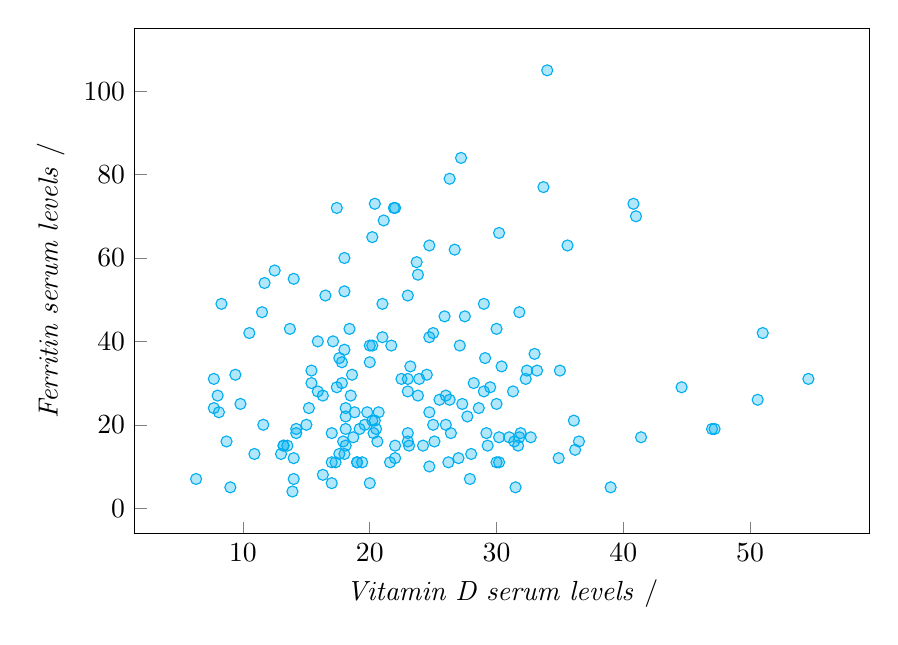
\begin{tikzpicture}
		\begin{axis}[scatter/classes={
			a={mark=*,cyan, fill opacity=0.3}},
			width=0.9\textwidth,
			height=8cm,
			xlabel = \textit{Vitamin D serum levels} $\si{\nano\gram/\milli\liter}$,
         	ylabel = \textit{Ferritin serum levels} $\si{\nano\gram/\milli\liter}$,
         	ytick pos=left,
         	xtick pos=left]
			\addplot[scatter,only marks,
				scatter src=explicit symbolic]
				coordinates {
					(20,6) [a]
					(8,27) [a]
					(23.8,56) [a]
					(7.7,31) [a]
					(11.7,54) [a]
					(8.1,23) [a]
					(21.7,39) [a]
					(12.5,57) [a]
					(11.6,20) [a]
					(32.3,31) [a]
					(22.5,31) [a]
					(25,42) [a]
					(30.2,66) [a]
					(31.8,47) [a]
					(16.3,27) [a]
					(17,6) [a]
					(10.9,13) [a]
					(31.4,16) [a]
					(18.4,43) [a]
					(27.1,39) [a]
					(29.5,29) [a]
					(13.5,15) [a]
					(26.3,79) [a]
					(30.4,34) [a]
					(36.2,14) [a]
					(31.9,18) [a]
					(31.7,15) [a]
					(28.2,30) [a]
					(35.6,63) [a]
					(36.5,16) [a]
					(23.2,34) [a]
					(21.6,11) [a]
					(20.4,73) [a]
					(35,33) [a]
					(7.7,24) [a]
					(16.3,8) [a]
					(13.9,4) [a]
					(26.7,62) [a]
					(15.9,40) [a]
					(27.7,22) [a]
					(28.6,24) [a]
					(41,70) [a]
					(23,51) [a]
					(27.2,84) [a]
					(22,12) [a]
					(17.3,11) [a]
					(18.1,22) [a]
					(17.9,16) [a]
					(6.3,7) [a]
					(16.5,51) [a]
					(20.4,21) [a]
					(23.7,59) [a]
					(25.5,26) [a]
					(31.3,28) [a]
					(32.4,33) [a]
					(24.7,41) [a]
					(21.1,69) [a]
					(26.4,18) [a]
					(20.5,19) [a]
					(30.2,11) [a]
					(18.7,17) [a]
					(18.6,32) [a]
					(11.5,47) [a]
					(18.1,15) [a]
					(29.3,15) [a]
					(34.9,12) [a]
					(54.6,31) [a]
					(15.9,28) [a]
					(10.5,42) [a]
					(14.2,18) [a]
					(23.1,15) [a]
					(32.7,17) [a]
					(13,13) [a]
					(24.7,23) [a]
					(20.3,18) [a]
					(30.2,17) [a]
					(20,39) [a]
					(24.2,15) [a]
					(17.8,30) [a]
					(24.5,32) [a]
					(29.2,18) [a]
					(13.2,15) [a]
					(20.2,65) [a]
					(13.7,43) [a]
					(8.3,49) [a]
					(9.4,32) [a]
					(13.2,15) [a]
					(20,35) [a]
					(17.8,35) [a]
					(20.6,16) [a]
					(41.4,17) [a]
					(31.5,5) [a]
					(27.3,25) [a]
					(44.6,29) [a]
					(24.7,10) [a]
					(14,7) [a]
					(33.7,77) [a]
					(29.1,36) [a]
					(27.9,7) [a]
					(26.3,26) [a]
					(24.7,63) [a]
					(14.2,19) [a]
					(20.2,39) [a]
					(20.7,23) [a]
					(15.4,30) [a]
					(21,41) [a]
					(26.2,11) [a]
					(17.6,13) [a]
					(33,37) [a]
					(23.8,27) [a]
					(23.9,31) [a]
					(30,43) [a]
					(18.8,23) [a]
					(18.1,19) [a]
					(21.9,72) [a]
					(25.9,46) [a]
					(27.5,46) [a]
					(19.8,23) [a]
					(15.4,33) [a]
					(50.6,26) [a]
					(19.4,11) [a]
					(25.1,16) [a]
					(25,20) [a]
					(18,13) [a]
					(17,11) [a]
					(39,5) [a]
					(23,18) [a]
					(17,18) [a]
					(23,28) [a]
					(30,25) [a]
					(18,38) [a]
					(14,55) [a]
					(14,12) [a]
					(23,16) [a]
					(15,20) [a]
					(19,11) [a]
					(26,27) [a]
					(22,15) [a]
					(29,28) [a]
					(26,20) [a]
					(18,52) [a]
					(23,31) [a]
					(34,105) [a]
					(47,19) [a]
					(51,42) [a]
					(18,60) [a]
					(19,11) [a]
					(22,72) [a]
					(30,11) [a]
					(28,13) [a]
					(21,49) [a]
					(29,49) [a]
					(27,12) [a]
					(31,17) [a]
					(17.1,40) [a]
					(20.2,21) [a]
					(31.8,17) [a]
					(40.8,73) [a]
					(17.4,29) [a]
					(8.7,16) [a]
					(17.4,72) [a]
					(36.1,21) [a]
					(19.2,19) [a]
					(47.2,19) [a]
					(33.2,33) [a]
					(9,5) [a]
					(18.1,24) [a]
					(17.6,36) [a]
					(9.8,25) [a]
					(18.5,27) [a]
					(19.6,20) [a]
					(15.2,24) [a]
				};
		\end{axis}
	\end{tikzpicture}
\caption{Scatter plot of Vitamin D and Ferritin serum levels.}
\label{fig:scatterplot_VitD_Ferritin}
\end{figure}

%Begin Table on Vitamin D and Ferritin
\begin{table}[H]
   \centering
   \begin{footnotesize}
   \begin{tabular}{c l c c c c | r}
   	  & & \multicolumn{3}{c}{Ferritin deficiency} & \\
   	  \cline{3-6}
       & & Absent & Mild & Moderate & Severe & Total\\
      \hline
       \parbox[t]{0.6cm}{\multirow{3}{*}{\rotatebox[origin=c]{90}{\begin{scriptsize}\begin{tabular}[t]{@{}c@{}}Vitamin D\\deficiency\end{tabular}\end{scriptsize}}}} & Absent & 68 (39.53\%) & 23 (13.37\%) & 10 (5.81\%) & 4 (2.33\%) & 105 (61.05\%)\\
       & Mild & 32 (18.60\%) & 11 (6.40\%) & 10 (5.81\%) & 4 (2.33\%) & 57 (33.14\%)\\
       & Moderate & 7 (4.07\%) & 1 (0.58\%) & 0 (0.00\%) & 2 (1.16\%) & 10 (5.81\%)\\
      \hline
       & Total & 107 (62.21\%) & 35 (20.35\%) & 20 (11.63\%) & 10 (5.81\%) & 172 (100.00\%)\\
   \end{tabular}
   \caption{Frequencies and percentages of ferritin and vitamin D deficient children in our population.}
    \label{tab:VitDFerritin}
    \end{footnotesize}
\end{table}

Then, we further studied anemias, by running a \textit{logistic regression}. Anemia was considered as a dichotomous variable (a children was either anemic or he wasn't), and so was done for parasitic infections, MCV and ferritin serum levels. We found that anemia is negatively correlated with MCV levels ($z=-3.18$, $p>|z|=0.001$ with a $CI_{95\%} =[0.75,0.93]$) (this stands out in Table \ref{tab:TODO} very well). Out of 22 anemias, 9 also had a pathological MCV ($\sim 41\%$); only 11\% of non anemic children presented a pathological MCV value.\\
There weren't any other statistically relevant correlations amongst the listed variables.

%TODO
%Insert Tab HB-MCV (TAB 4) HERE e aggiungi reference sopra.

Because of this strong relation between low-MCV and low-haemoglobin, we decided to consider the population with these two parameters offset and try to find out more (3.25\%). We found that there was a positive correlation between ferritin low serum levels and the a low-MCV anemia, confirming the high prevalence of iron-deficiency in our population. This was confirmed at the \textit{Fisher's exact test} ($p=0.001$). Table \ref{tab:TODO} shows our data for this consideration.\\
This low-MCV low-haemoglobin population all came from Asia ($n=5$, $\sim 55\%$) and Eastern Europe ($n=4$, $\sim 44\%$). This was statically significant, with a Fisher's exact test result of $p=0.033$. In particular, the only involved countries were India ($n=5$, $\sim 55\%$), in Asia, and Russia ($n=2$, $\sim 22\%$) and Bulgaria ($n=2$, $\sim 22\%$), in Eastern Europe.

%TODO
%Insert Tab Ferritin-MCV+HB (TAB 5) HERE e aggiungi reference sopra.

Moreover, we tried to look even closer at anemias and parasitic infections: the variables were found still to be independent at \textit{Fisher's exact test} ($p=0.935$). No correlation was found (leaving us pretty surprised) neither between anemia and group 1 and 2 gastrointestinal infestations, with a \textit{Fisher's exact test} result of $p=0.205$ and $p=0.669$ respectively. Tables \ref{tab:TODO}, \ref{tab:TODO}, and \ref{tab:TODO} summarize our findings.\\
On the other hand, we found a positive correlation between pathological ferritin and group 1 parasitic infection, with a \textit{Fisher's exact test} result of $p=0.003$. This finding is in accordance with our definitions of group 1 and 2 parasites, since the first commonly express their infections through gastrointestinal bleeding.

%TODO
%Insert Tab Parassiti-Anemia (TAB 3) HERE e aggiungi reference sopra.

%TODO
%Insert Tab Parassiti-Anemia (TAB 6 e 7) HERE e aggiungi reference sopra.

Lastly, we tried a \textit{logistic regression} on low height for age, anemia, group 1 and 2 parasitic infections, Mantoux test results, and vitamin D serum levels, but no statistically relevant result was found. We believe that through a bigger sample size anemias, Mantoux test results, and group 2 parasitic infections would have found a rather strong correlation with pathological height, as a chronic illness indicator.
